\section{Actor-Critic Methods}
\raggedbottom 
Many different approaches to different kind of reinforcement learning problems exist. 
Dynamic programming methods can compute optimal policies, however a perfect model of the environment as MDP is required.
Monte-Carlo methods on the other hand can estimate value functions and discover optimal policies by averaging over sampled trajectories.

\subsection{TD-Learning}

\cite{Sut98} describes \textit{temporal difference} (TD) learning as one of the central ideas in reinforcement learning.
TD learning combines dynamic programming with Monte-Carlo methods to learn eather \textit{state-values: V(s)} or \textit{state-action values: Q(s, a)} which are given as:

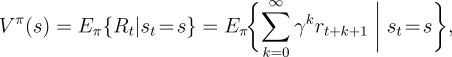
\includegraphics[scale=0.5]{bilder/valfct.png}

and

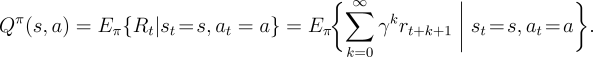
\includegraphics[scale=0.5]{bilder/qvalfct.png}

respectively, where \textit{$E_{\pi}$} denotes the expected \textit{return}, which is the accumulated discounted reward starting from a state or state-action pair, following the policy $\pi$

One of the most important TD-learning methods is Q-Learning. 
It is used to approximate the state-action value function:

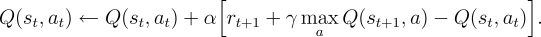
\includegraphics[scale=0.5]{bilder/qlearning1.png}

The agent can then direcly choose the action which is expected to give the best total reward.
The $\epsilon$-greedy policy is usually applied, which uses eather the best estimated action or a random policy to decide the next action, depending on the $\epsilon$ value, which is gradually lowered over the learning period, to reach optimal behaviour while ensuring sufficient exploration.
Following algorithm is given by \citet{Sut98}

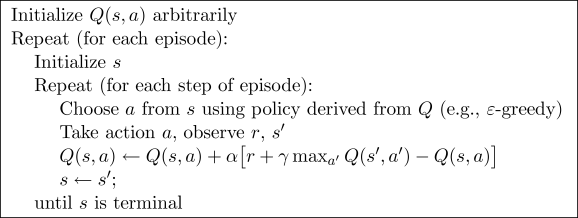
\includegraphics[scale=0.5]{bilder/qlearning2.png}
\pagebreak
\subsection{Critic-Only Methods}

The shown Q-learning algorith or SARSA are popular critic-only methods.

Critic-only methods learn state-action values. They do not contain an explicit function for the policy, but rather derive it from the learned state-action values by acting greedy on the Q-Values.

By only using a critic a low variance estimate of the expected returns is achieved, however the methods suffer from being biased and can be problematic in terms of convergence.

\subsection{Actor-Only Methods}

Onlike critic-only methods, actor only methods do not learn any state or state-action values.
Instead they perform optimization directly on the policy.
Usually a stochastic and parameterized policy $\pi_\theta$ is used.

Policy gradient methods like REINFORCE change the policy in order to maximize the average reward at a given timestep by performing a gradient ascent step. \citep{Williams1992}
Given a performance (average reward per timestep) J and a policy which is parameterized by $\theta$ we can denote the gradient as
\begin{center}
$\Delta \theta = \alpha \frac{\partial J}{\partial  \theta}$
\end{center}

where $\alpha$ denotes the step size.


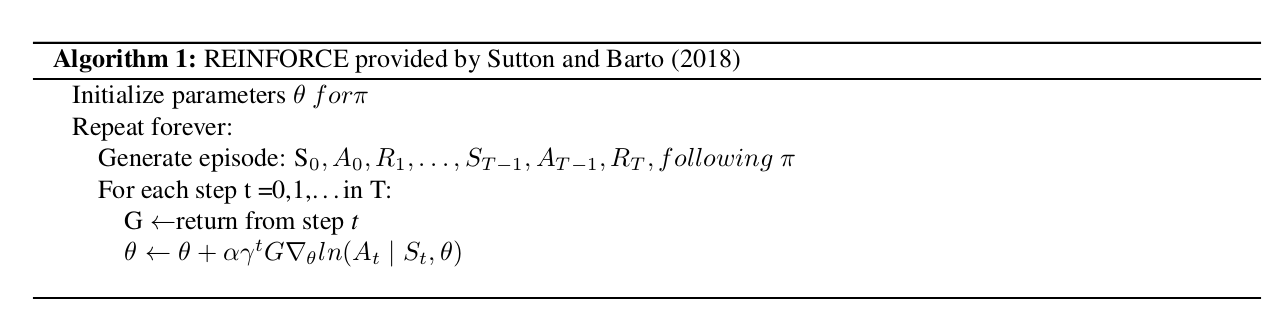
\includegraphics[scale=0.4]{bilder/REINFORCE.png}

In contrast to value based approaches, policy gradient methods provide strong convergence to at least a local maximum.
On top of that, actor methods are applicable on continuus action spaces.
 \citep{Sutton00policygradient}
Actor-only methods however suffer from a large variance of the gradient. Compared to critic-only methods their learning process is significantly slowed down. \citep{Grondman12}
 

\subsection{Actor-Critic Methods}

Actor-critic methods tackle the problem of high variance in policy gradient methods with the use of a critic. 
\pagebreak

\subsection{Asynchronous Advantage Actor Critic (A3C)}

In general we call an algorithm on policy, if the data used in the policy update was sampled under the same policy. The sequence of observed data encountered by an RL agent is strongly correlated and non-stationary \citep{A3C}. This can have a negative influence on the learning process.

Previous methods usually approached this problem by using randomly selected samples from a replay memory \citep{mnih2015atari}

Training an agent comes with a high demand for computational power. To achieve feasible training times, former algorithms heavily relied on a strong GPU.

The asynchronous advantage actor critic(A3C) algorithm solves both problems, by training simultaneously on multiple environment.
Each learner samples trajectories and computes gradients. Those gradients are then applied to the shared parameters. 
After each global update step, the local parameters are synchronized.
This method enables efficent CPU computation, rather than using a GPU.
The core idea is, that each agents environement is in a very different state, thus reducing the correlation of the samples.
 
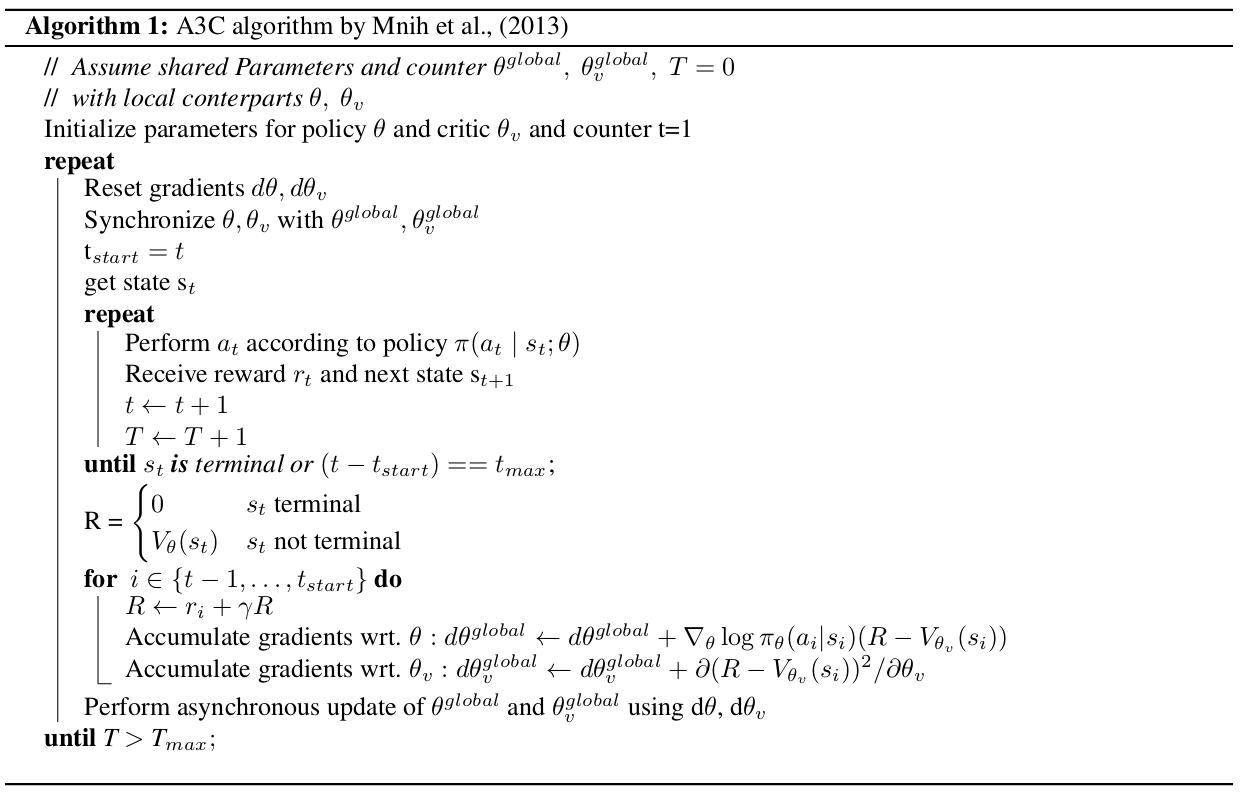
\includegraphics[scale=0.3]{bilder/aaac.png}
